\chapter{Arquitetura do \textit{Software}}\label{cap:arquitetura}

O \textit{software} desenvolvido é uma ferramenta, e ao longo deste capítulo ele
é referido simplesmente por "a ferramenta".  Este capítulo descreve como a
ferramenta interage com os outros \textit{softwares} em uso na competição.  Os
seguintes são de relevância para o entendimento da arquitetura escolhida:

\begin{itemize}
  \item ssl-vision: desenvolvido pela comunidade e de uso oficial na competição
    para processamento das imagens da câmera nas partidas e distribuição pela
    rede dos dados processados (estado do jogo);
  \item grSim: desenvolvido pela comunidade e amplamente usado pelas equipes
    para simular o ambiente das partidas, o protocolo usado para enviar o estado
    pela rede é identico ao do ssl-vision;
  \item pyroboime: também chamado de core desenvolvido pela RoboIME, atualmente
    provê uma camada de abstração sobre a comunicação com o ambiente de jogo
    (real ou simulado) incluindo redução de ruído, planejamento de trajetória e
    controle.
\end{itemize}

% Para fins práticos o desenvolvimento ocorre com validações no simulador (grSim).
% O comportamento é compatível com as partidas oficiais.

A ferramenta está implementada em C++11 (revisão recente de C++ suportada pela
maioria dos compiladores modernos).

\section{Comunicação com Componentes Externos}

\begin{figure}[H]
  \centering
  %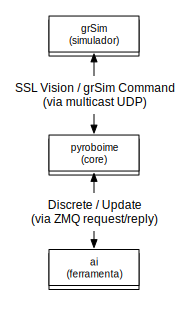
\includegraphics[height=10cm]{communication}
  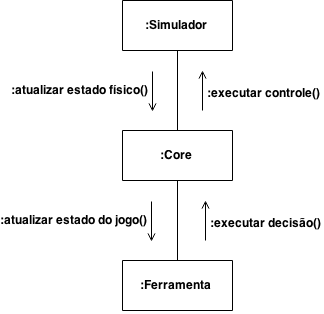
\includegraphics[height=8cm]{uml_comm}
  % TODO[jansegre]: fazer diagrama certo ou mudar o nome
  \caption{Diagrama de comunicação entre os componentes.}\label{fig:arch_comm}
\end{figure}

A Figura~\ref{fig:arch_comm} representa como os componentes se comunicam.  A
ferramenta se comunica apenas com o pyroboime para aproveitar todas as
funcionalidades necessárias que fogem ao escopo desse trabalho.  Por isso o foco
do desenvolvimento está concentrado em atender diretamente os objetivos.

As mensagens trocadas entre a ferramenta e o core (\textit{pyroboime}) são
codificadas com o \textit{Protobuf}~\cite{protobufdocs}, uma biblioteca bem
estabelecida que também é usada nos protocolos oficiais da competição.  Desse
modo o \textit{overhead} de comunicação é baixo, não é necessário introduzir uma
dependência ou codificação manual no core e é possível que versões futuras sejam
retrocompatíveis.

São dois tipos de mensagens:

\begin{itemize}
  \item atualização do estado: sentido do core para a ferramenta, codificadas
    com a mensagem UpdateMessage, descreve todas as informações necessárias para
    criar um estado novo;
  \item comando de ações: sentido ferramenta para o core, codificadas com a
    mensagem CommandMessage, descreve a ação que cada agente (robô) deve
    realizar.
\end{itemize}

%As especificações de ambas as mensagens se encontram no Anexo~\ref{att:protos}.

As mensagens são transmitidas em um socket ZMQ (\textit{ZeroMQ}~\cite{zmqdocs},
uma biblioteca de transmissão de dados na rede) visando a extensibilidade da
ferramenta, pois com tal biblioteca é possível distribuir mensagens entre vários
nós de forma confiável (característica desejável para um sistema distribuido)
além de provêr confiabilidade e auto-reconexão para o uso atual.

O modo de transmissão é o \textit{request-reply}, em que a ferramente age como
servidor respondendo as requisições do core. Esse modelo é composto por
atualizações cuja a resposta deve ser o comando a ser executado naquele estado
requisitado.  Na prática a ferramenta irá transmitir o comando mais recente,
que se encontra em seu \textit{buffer}, descrito brevemente no
Seção~\ref{sec:threads}.

\section{\textit{Threads} do Sistema}\label{sec:threads}

\begin{figure}[H]
  \centering
  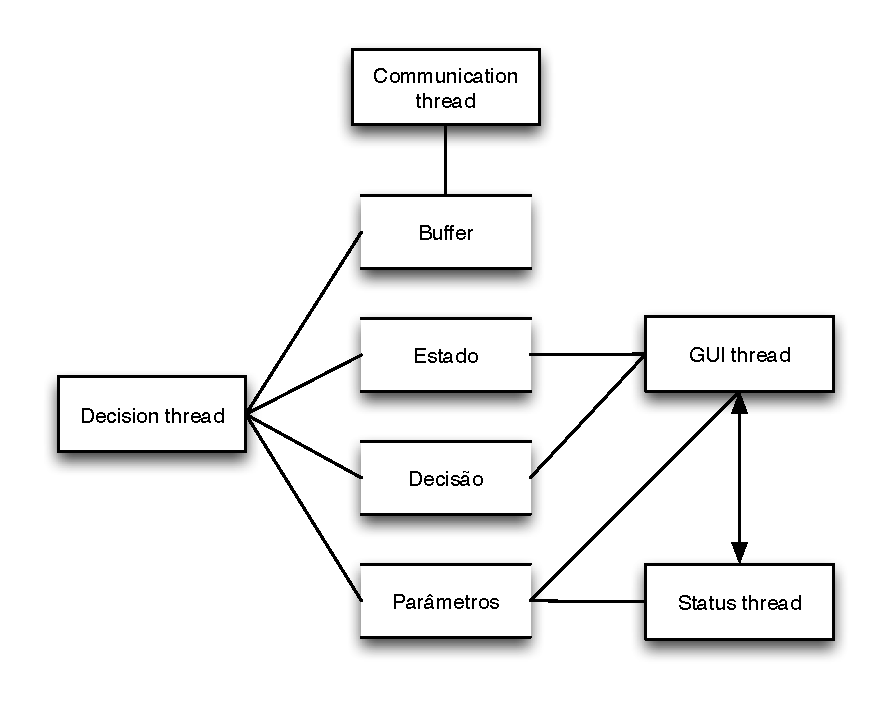
\includegraphics[height=10cm]{threads}
  \caption{Diagrama de relação entre \textit{threads} e
  dados.}\label{fig:arch_threads}
\end{figure}

A ferramenta está implementada em quatro \textit{threads} fixas de acordo com a
Figura~\ref{fig:arch_threads}.  A separação foi motivada por:

\begin{itemize}
  \item interface gráfica responsiva ao usuário;
  \item taxa de tomada de decisão poder ser mais lenta que a taxa de
    atualização do estado, portanto a comunicação tem sua própria
    \textit{thread} que escreve e lê de um buffer compartilhado pela
    \textit{thread} de tomada de decisão;
  \item certas informações devem ser coletadas periódicamente para atualizar
    alguns parâmetros e exibidas para o usuário.
\end{itemize}

\section{Interface Gráfica}

É importante destacar o fato que a interface gráfica tem um papel muito
importante na ferramenta.  Ela possibilita que um usuário não programador
modifique, em tempo de execução, um conjunto de configurações que modifica, com
uma grande amplitude, o comportamento do time controlado.  A interface visa
prover uma representação de simples compreensão do estado do jogo e de como as
várias configurações podem afetar o comportamento.  Maiores detalhes sobre a
interface em si são discutidos na Seção~\ref{sec:gui}.  Esta seção aborda
a arquitetura implementada que provê a interface.

A Figura~\ref{fig:arch_gui} mostra como os componentes interagem.  Em mais
detalhes, esses componentes são:

\begin{itemize}
  \item GLFW: biblioteca que abstrai as APIs nativas de manipulação de janelas e
    de eventos de mouse e teclado.  Além de fornecer contextos OpenGL.  Seu uso
    é importante pois permite que a ferramenta seja compilada sem alteração para
    diferentes sistemas operacionais.\footnote{Fato que ocorreu durante todo o
      desenvolvimento.  A ferramenta foi desenvolvida principalmente no OS X, e
      em parte no Ubuntu (distribuição de Linux).  Além disso, um serviço de
      integração (Travis CI) foi usado para validar a compilação no Ubuntu.
    Embora desejável, não houve tentativa de compilação no Windows.} (biblioteca
    disponível em \cite{glfwdocs})
  \item OpenGL: API de renderização 2D e 3D.  Seu uso se restringe a
    renderizações no plano (2D).  É usada para desenhar todos os objetos que
    representam estados, decisões e alguns artefatos auxiliares, além de ser
    usado para prover o \textit{backend} de renderização do ImGui. (API
    disponível em \cite{opengldocs})
  \item ImGui: Biblioteca leve de \textit{widgets} usada para criar janelas
    internas, botões, barras de configuração deslizantes, caixas de seleção,
    entre outros \textit{widgets}.  Como não possui dependências é necessário
    prover um \textit{backend} de renderização.  Outra vantagem é ser orientada
    a "modo imediato", na prática isso significa que, por exemplo, desenhar um
    botão é uma única chamada de função, sem a necessidade de estruturação e
    gerenciamento manual dos \textit{widgets}. (biblioteca disponível em
    \cite{imguigithub})
\end{itemize}

\begin{figure}[H]
  \centering
  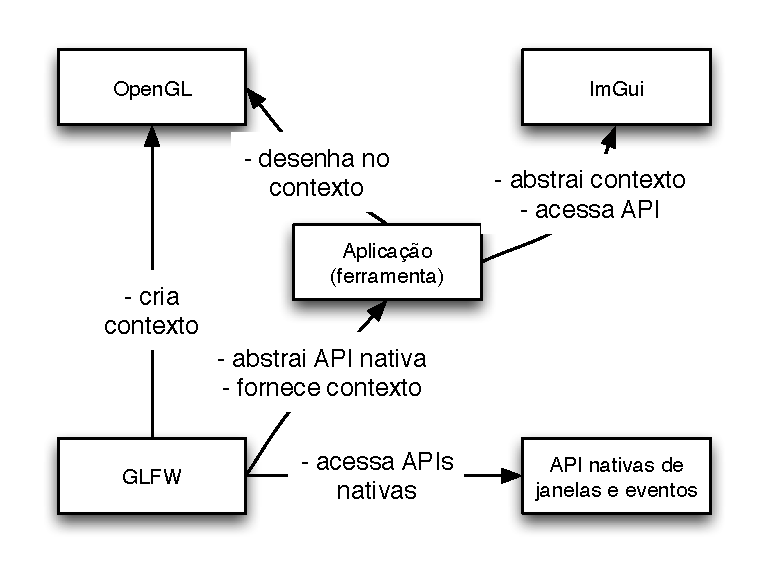
\includegraphics[height=10cm]{gui}
  % TODO[jansegre]: Fazer diagrama de compontes UML
  \caption{Diagrama de relação entre componentes gráficos}\label{fig:arch_gui}
\end{figure}

% vim: tw=80 et ts=2 sw=2 sts=2 ft=tex
